\input{../../../Commun/macros_TD.tex}

\title{Cellular Biology \& Biochemistry for Engineers\\TD2}
\author{Harald \textsc{Hirling}}
\date{29 sept. 2015}

\begin{document}
\maketitle

\section*{14)}

The worm is pretty simple and good for this study. Drosophila is another choice.

\section*{15)}

Anatomy. DNA similarity.

\section*{16)}

No. Only the complexity of the genes expression matters.

\section*{17)}

The size of the electronic cloud, the size of the nucleus (which repulse each other).

\section*{18)}
A: 7; 
B: 2; 
C: 5; 
D: 1;
E: 6

\section*{19)}

Sugar is hydrophilic.

Salt separate into two ions which dissolve easily since water is polar.

\section*{20)}

Nnnope.
\begin{figure}[!ht]
    \centering
    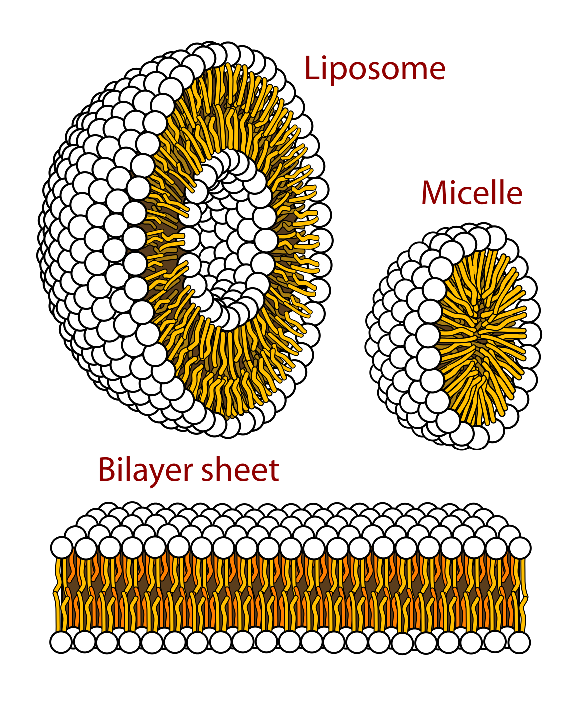
\includegraphics[scale=0.5]{figures/lipids}
    \caption{Arrangement of lipids in aqueous medium}
\end{figure}

\FloatBarrier

\section*{21)}

There is more $H^+$ ($H_3O^+$) in pH6. We need to add protons to change pH9 in pH6.

\section*{22)}

Sugar (pentose), phosphate and nitrogenous base.

\section*{23)}

Phospholipids are amphipathics.

Hydrophilic: likes water.

Hydrophobic: dislikes water.

amphipathics: hydrophilic and hydrophobic.

\section*{24)}

They all are acids ($COOH$) and have a amine group ($N_20$). 

There are different characteristics: polar (hydrophilic), apolar (hydrophobic), acid, base.

\section*{25)}



\bibliographystyle{alpha}
\bibliography{bibliography}
\nocite{*}

\end{document}





